%%%%%%%%%%%%%%%%%%%%%%%%%%%%%%%%%%%%%%%%%%%%%%%%%%%%%%%%%%%%%%%%%%%%%
%% This is a (brief) model paper using the achemso class
%% The document class accepts keyval options, which should include
%% the target journal and optionally the manuscript type.
%%%%%%%%%%%%%%%%%%%%%%%%%%%%%%%%%%%%%%%%%%%%%%%%%%%%%%%%%%%%%%%%%%%%%
\documentclass[journal=cmatex,manuscript=article]{achemso}

%%%%%%%%%%%%%%%%%%%%%%%%%%%%%%%%%%%%%%%%%%%%%%%%%%%%%%%%%%%%%%%%%%%%%
%% Place any additional packages needed here.  Only include packages
%% which are essential, to avoid problems later. Do NOT use any
%% packages which require e-TeX (for example etoolbox): the e-TeX
%% extensions are not currently available on the ACS conversion
%% servers.
%%%%%%%%%%%%%%%%%%%%%%%%%%%%%%%%%%%%%%%%%%%%%%%%%%%%%%%%%%%%%%%%%%%%%
\usepackage[version=3]{mhchem} % Formula subscripts using \ce{}
\usepackage[T1]{fontenc}       % Use modern font encodings

\usepackage{amssymb}
\usepackage{amsmath}

\usepackage{color}
\def\blue#1{\textcolor[rgb]{0,0,1}{#1}}
\def\red#1{\textcolor[rgb]{1,0,0}{#1}}
\usepackage[normalem]{ulem}
\usepackage{comment}

\newcommand*\mycommand[1]{\texttt{\emph{#1}}}


\author{Author1}
\affiliation[A]
{Department of Mechanical Science and Engineering, University of Illinois at Urbana-Champaign, 1206 W. Green Street, Urbana, Illinois 61801, United States}
\alsoaffiliation[B]
{Materials Research Laboratory, University of Illinois at Urbana-Champaign, Urbana, Illinois 61801}

\author{Author2}
\affiliation[C]
{Department of Materials Science and Engineering and Materials Research Laboratory, University of Illinois at Urbana-Champaign, 1304 W. Green Street, Urbana, Illinois 61801, United States}

\author{Author3}
\affiliation[A]
{Department of Mechanical Science and Engineering, University of Illinois at Urbana-Champaign, 1206 W. Green Street, Urbana, Illinois 61801, United States}



\title{ insert your title here }


%\abbreviations{... }
%\keywords{First principles, density functional theory, perovskite, brownmillerite, strontium titanate}


\begin{document}


%\begin{tocentry}
%\includegraphics{figure_TOC.png} 
%\end{tocentry}

%%%%%%%%%%%%%%%%%%%%%%%%%%%%%%%%%%%%%%%%%%%%%%%%%%%%%%%%%%%%%%%%%%%%%
%% The abstract environment will automatically gobble the contents
%% if an abstract is not used by the target journal.
%%%%%%%%%%%%%%%%%%%%%%%%%%%%%%%%%%%%%%%%%%%%%%%%%%%%%%%%%%%%%%%%%%%%%

\newpage
\begin{abstract}
\blue{[put your abstract here.]}
\end{abstract}

%%%%%%%%%%%%%%%%%%%%%%%%%%%%%%%%%%%%%%%%%%%%%%%%%%%%%%%%%%%%%%%%%%%%%
%% Figure 1
%%%%%%%%%%%%%%%%%%%%%%%%%%%%%%%%%%%%%%%%%%%%%%%%%%%%%%%%%%%%%%%%%%%%%

\newpage

\begin{figure*}[!hbtp] %*
\centering
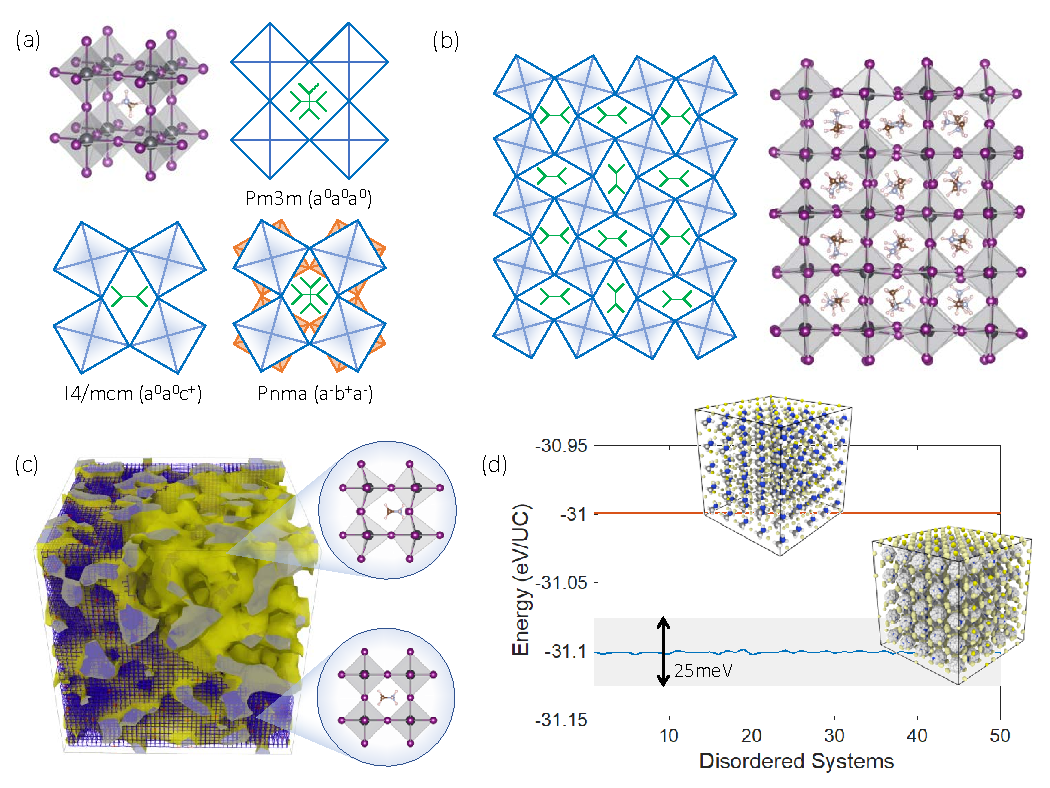
\includegraphics[width=6in]{Figure1.pdf}
\caption{\label{fig1} 
Types of structural disorder in hybrid perovskites: (i) random orientational disorder of $A$-site organic molecules, (ii) incommensurate tilings of the inorganic PbI$_6$ framework, and (iii) coexistence of different phases.
(a) The cubic prototype and two tilting modes of the PbI$_6$ framework, which lead to three phases. 
(b) Ideal tessellation of $M$-tilted motif, compared with the configuration generated from \emph{ab-initio} molecular dynamics, where incommensurate rotations can be identified.
(c) Coexistence of shape-preserving octahedra and incommensurate phases. The blue-colored frame denotes the lattice, and the yellow isosurface illustrates the boundary between regions of differing octahedral tiling. 
(d) Lattice energy of the ordered cubic phase (red) compared to 50 different disordered phases (blue) obtained \emph{via} slow cooling of independent configurations from molecular dynamics. The insets show the ordered pristine supercell versus 50 disordered snapshots plotted together. The energy differences amongst the disordered systems are within room temperature thermal fluctuations. (UC: unit cell for cubic perovskite.)
}
\end{figure*} %*


To learn: The purpose of this figure is to show the different typess of disorder that are present in hybrid organic/inorganic perovskites: molecular orientations, tilings of the octahedral framework, and phase coexistence. It also shows that different configurations sampled by  the system in time are thermodynamically equivalent at room temperature. 

%%%%%%%%%%%%%%%%%%%%%%%%%%%%%%%%%%%%%%%%%%%%%%%%%%%%%%%%%%%%%%%%%%%%%
%% Figure 2
%%%%%%%%%%%%%%%%%%%%%%%%%%%%%%%%%%%%%%%%%%%%%%%%%%%%%%%%%%%%%%%%%%%%%


\newpage

\begin{figure*}[!hbtp] %*
\centering
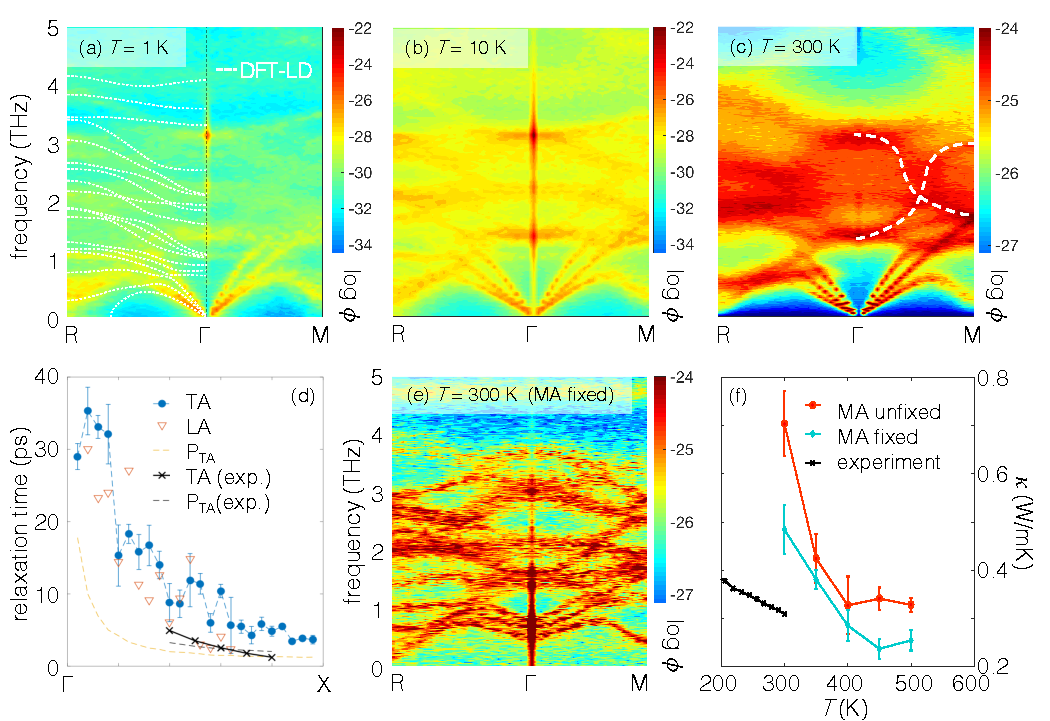
\includegraphics[width=6in]{Figure2.pdf}
\caption{\label{fig2} 
(a-c) Spectral energy density of dynamical modes in MAPbI$_3$ at different  temperatures from {\it ab-initio} molecular dynamics. 
The dotted white line for $T = 1^\circ$ K shows the lattice dynamics result for comparison. 
The band line-widths broaden as temperature increases. 
At $T=300^\circ$ K, the vibrational modes between 3-4 THz that are well-defined at low temperatures are now heavily blurred. 
%Instead, ``waterfall-like" modes are observed. 
(d) The modal relaxation time extracted from SED compared to recent experimental measurements \cite{gold2018acoustic}. 
The relaxation time is close to the wave period for each thermal carrier, suggesting the conventional phonon picture is not an adequate description of the carriers (see also Figure S1). %\ref{figS_mfp}
(e) Freezing the rotations of the MA molecules recovers the well-defined lattice dynamical modes, which suggests that interactions between the inorganic framework and sublattice MA orientational disorder are responsible for the loss of wave nature in (c).
(f) Thermal conductivity calculated via Green-Kubo formalism using classical molecular dynamics, with MA fixed and unfixed, compared with experiments \cite{kovalsky2017thermal}. 
}
\end{figure*} %*


To learn: The purposes of this Figure is to show that the phonon character of the vibrations of the hybrid organic/inorganic material disappears as the temperature and orientational disorder increase. 





%%%%%%%%%%%%%%%%%%%%%%%%%%%%%%%%%%%%%%%%%%%%%%%%%%%%%%%%%%%%%%%%%%%%%
%% The appropriate \bibliography command should be placed here.
%% Notice that the class file automatically sets \bibliographystyle
%% and also names the section correctly.
%%%%%%%%%%%%%%%%%%%%%%%%%%%%%%%%%%%%%%%%%%%%%%%%%%%%%%%%%%%%%%%%%%%%%
\newpage
\bibliography{mybib.bib}

\end{document}
